\chapter{SYSTEM DESIGN}
\section{Use Case Diagram}

Description:

	A use case diagram is the simplest representation of a user's interaction with the system and depicting the specifications of a use case. A use case diagram can define the different types of users of a system and the various ways that they interact with the system. They provide the simplified and graphical representation of what the system must actually do.The purpose of the use case diagrams is simply to provide the high level view of the system and convey the requirements.


\subsection{ Use-Case Diagram}
\begin{figure}[H]

\centering

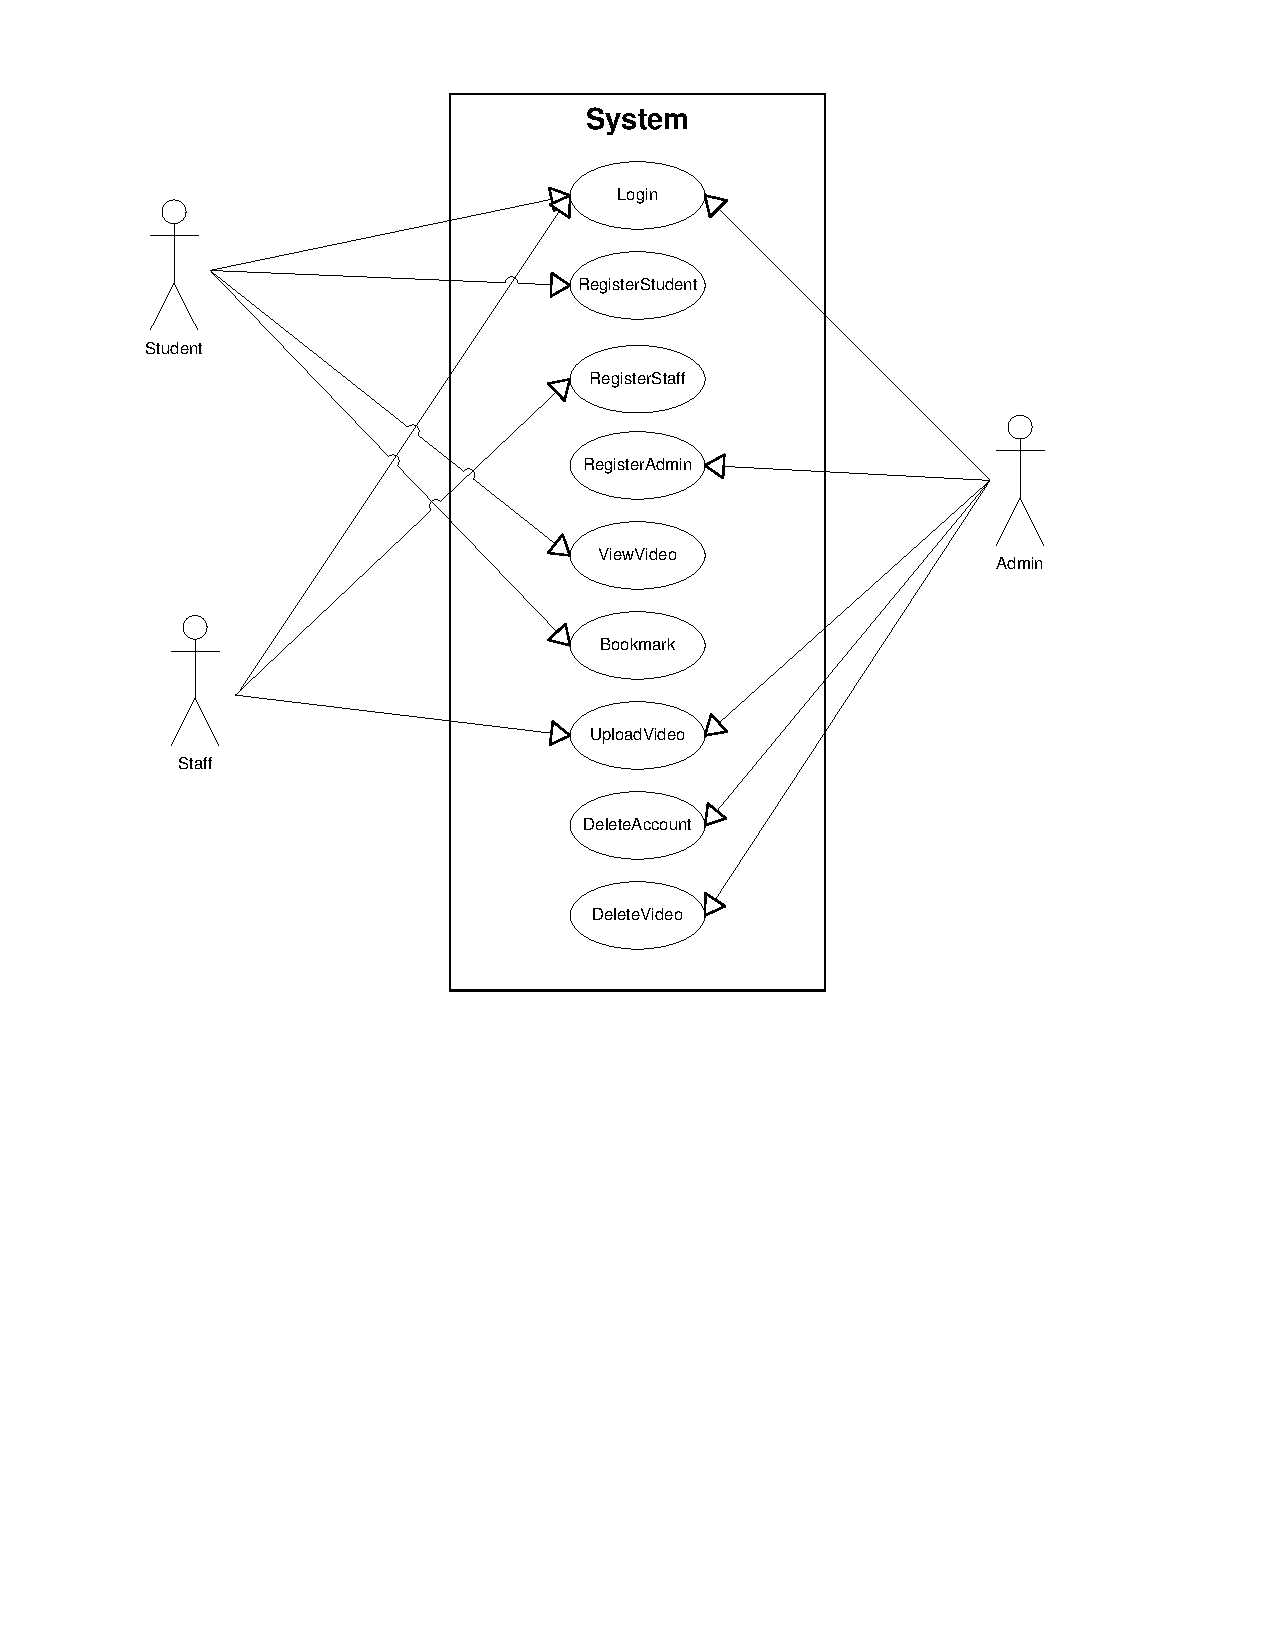
\includegraphics[width=5in]
{usecase1.pdf}
\caption{Use case diagram for Virtual Classroom.}
\end{figure}


\subsection{ Use-Case Scenario}
\begin{figure}[H]

\centering

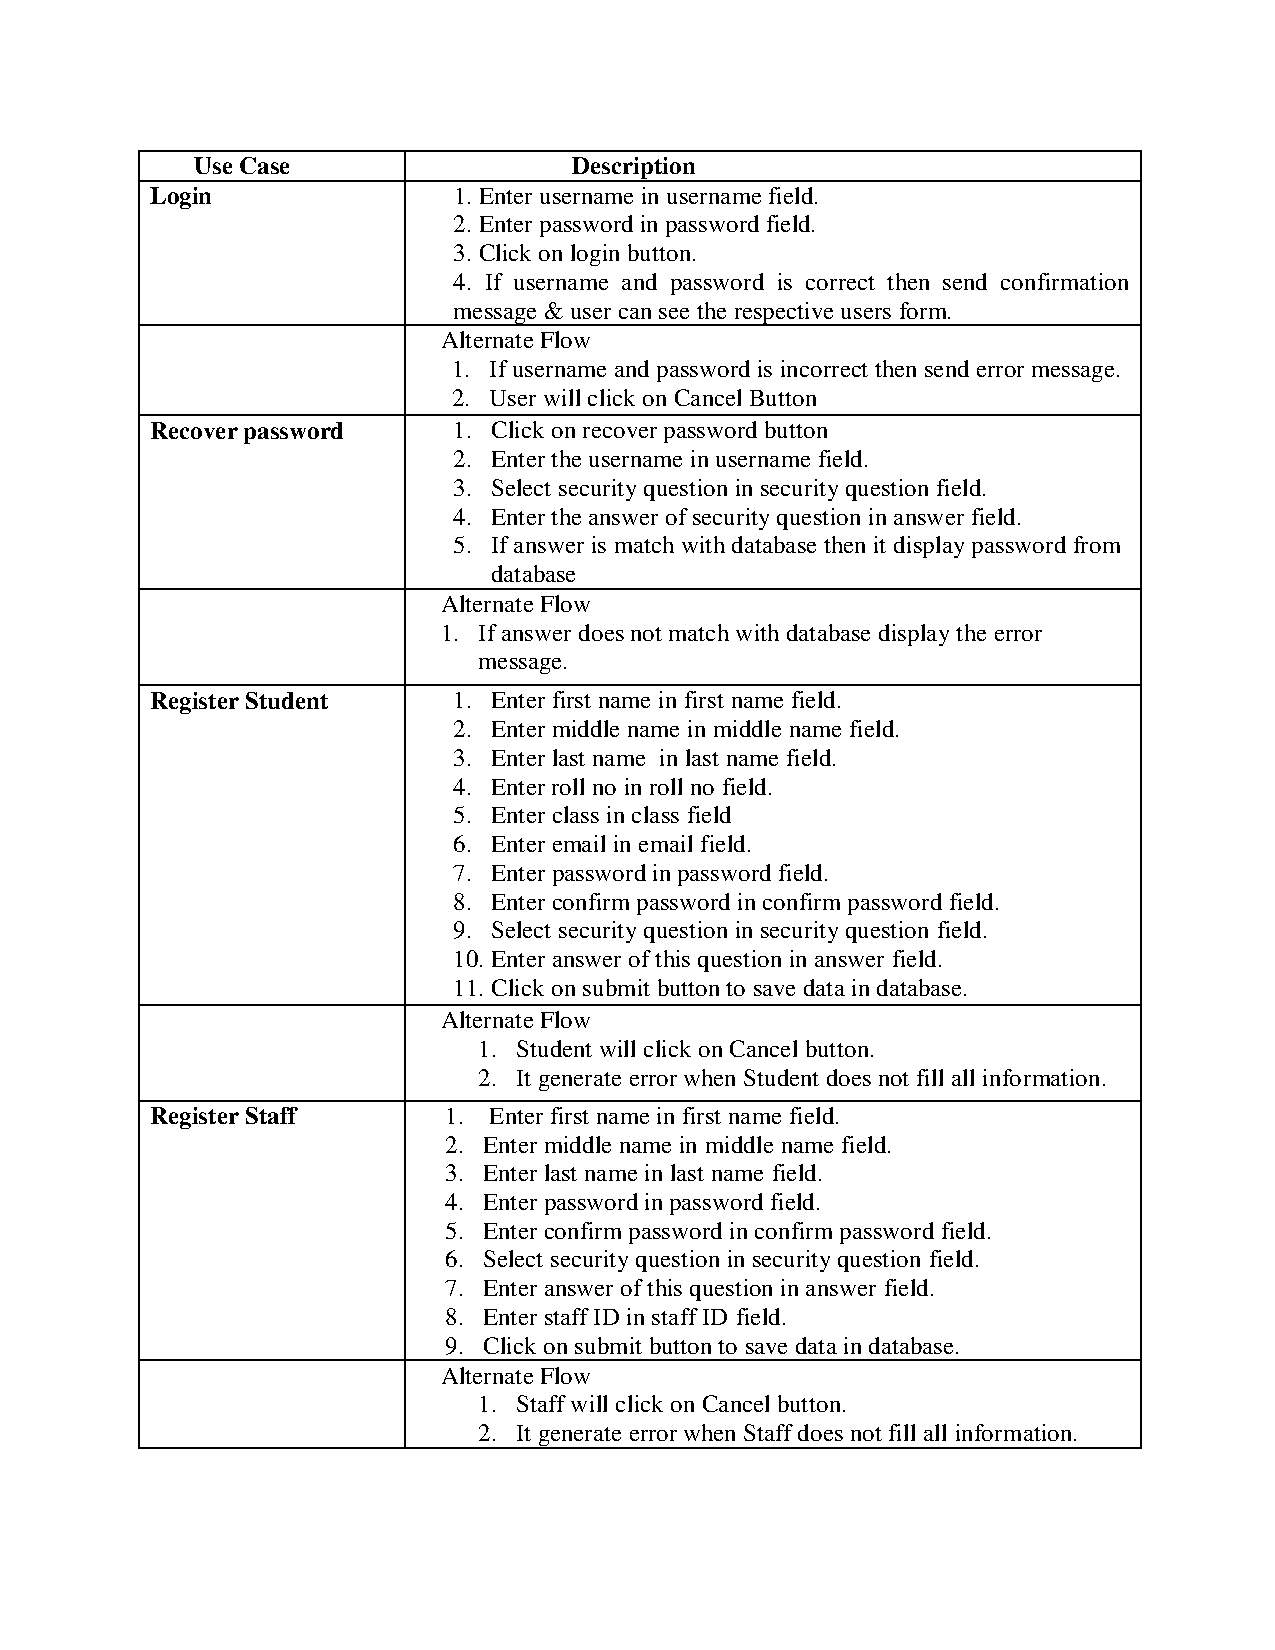
\includegraphics[width=5in]
{usecasescenario.pdf}
\caption{Use Case Scenario Table.}
\end{figure}

\section{Sequence Diagram}

A Sequence diagram is an interaction diagram that shows how processes operate with one another and in what order. It is a construct of a Message Sequence Chart. A sequence diagram shows object interactions arranged in time sequence. It depicts the objects and classes involved in the scenario and the sequence of messages exchanged between the objects needed to carry out the functionality of the scenario. Sequence diagrams are typically associated with use case realizations in the Logical View of the system under development. Sequence diagrams are sometimes called event diagrams or event scenarios.



\subsection{Sequence Diagrams for Login User:}

\begin{figure}[H]

\centering

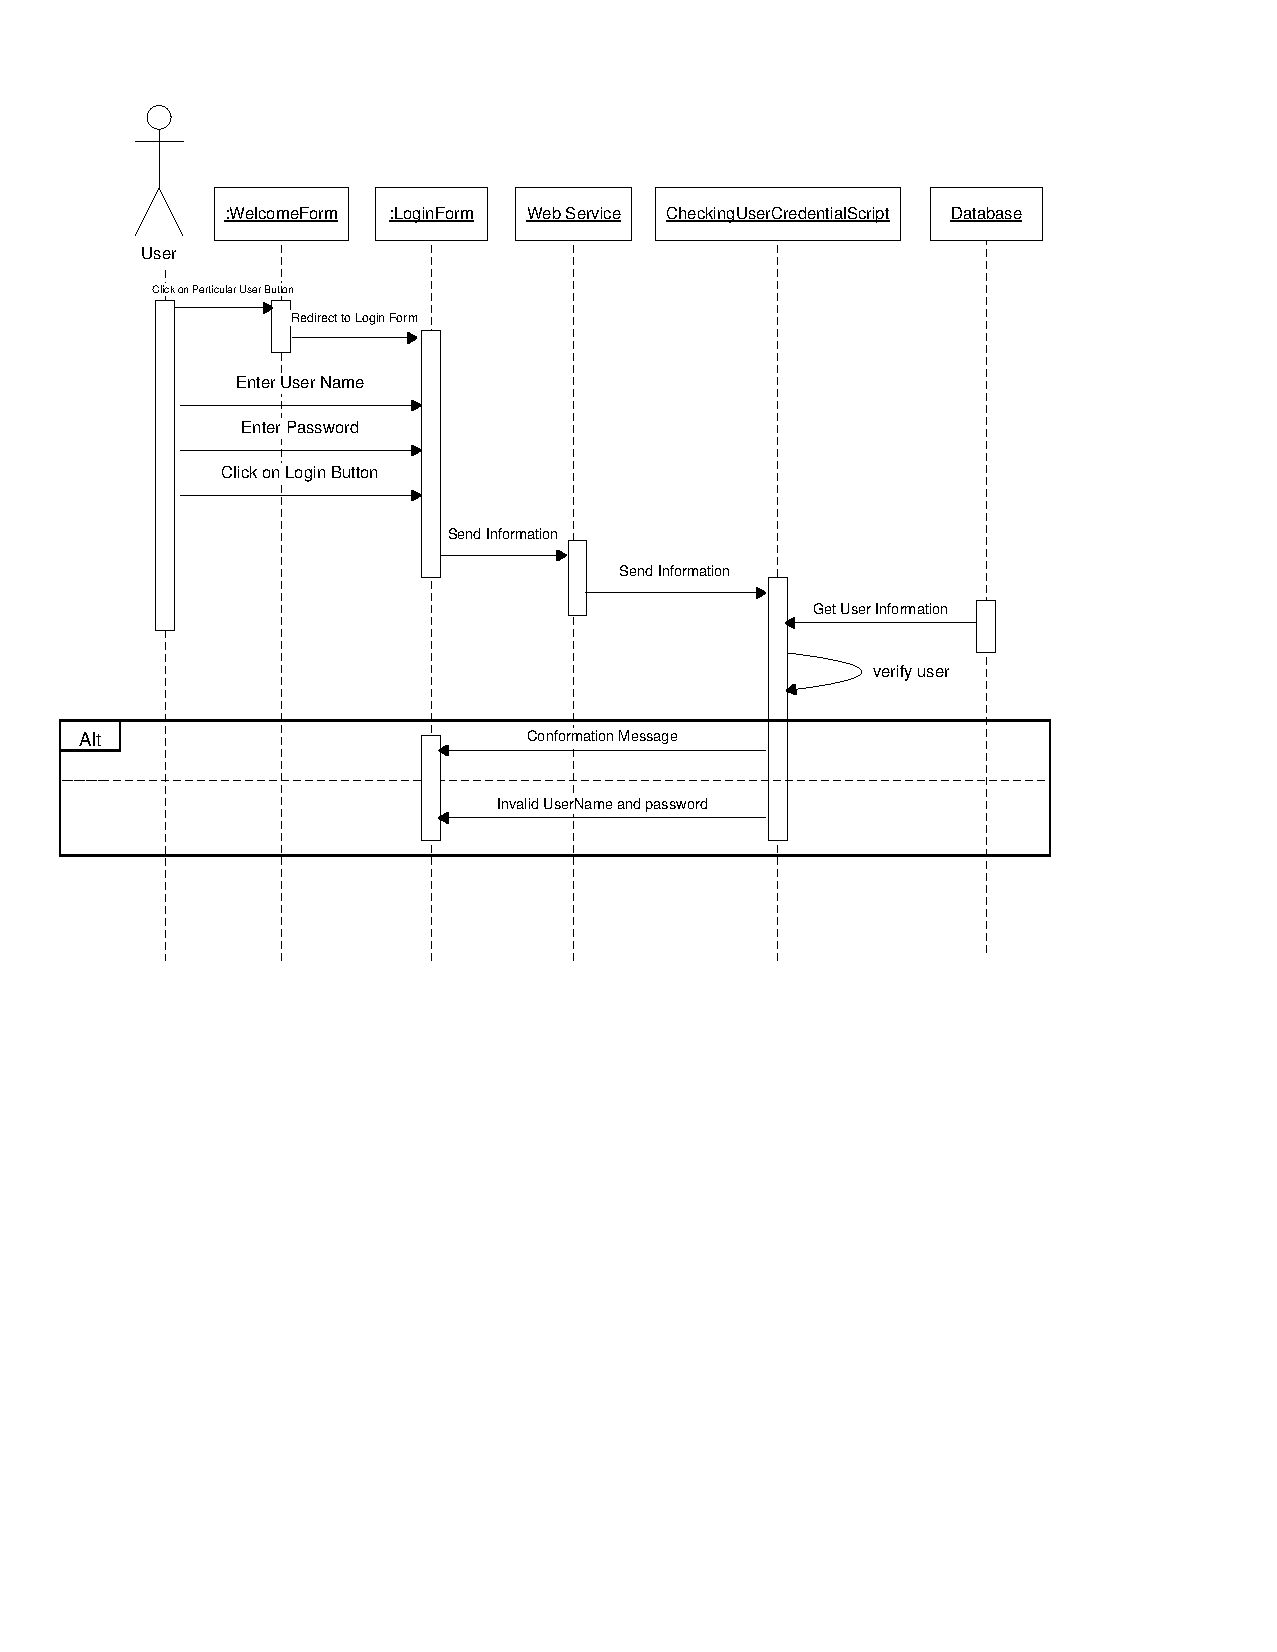
\includegraphics[width=5in]
{SDforLoginv1.pdf}
\caption{sequence diagram for User Login}
\end{figure}

 Above diagram shows the sequence of activities carried out when login is done. Using the above form student, staff as well as admin is able to login. 

\subsection{Sequence Diagrams for Recover Password:}

\begin{figure}[H]

\centering

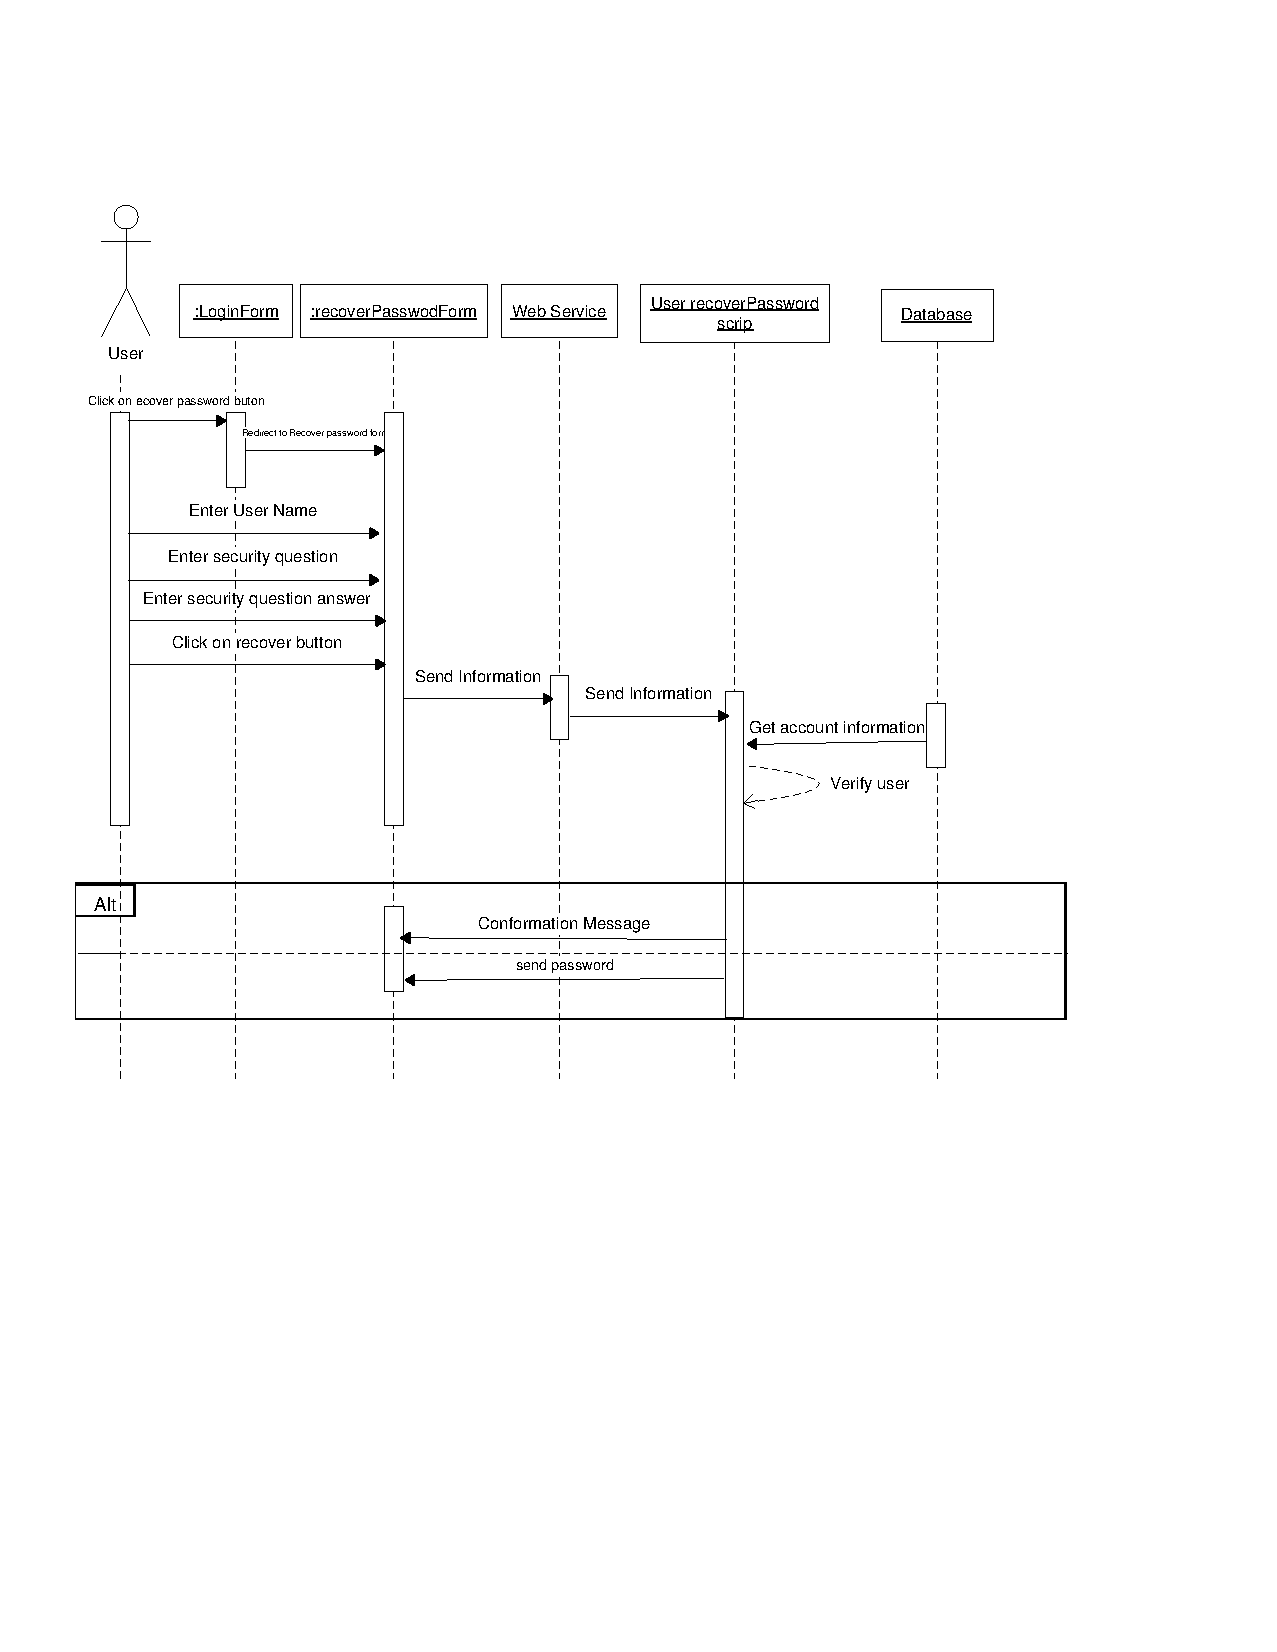
\includegraphics[width=5in]
{recoverpassword1.pdf}
\caption{sequence diagram for Recover Password}
\end{figure}

Above diagram shows sequence diagram for recover password. To recover password user choose security and answer. The answer given by user is compared with database. If answer matches then password is sent to user.

\subsection{Sequence Diagrams for Register Admin:}
\begin{figure}[H]

\centering

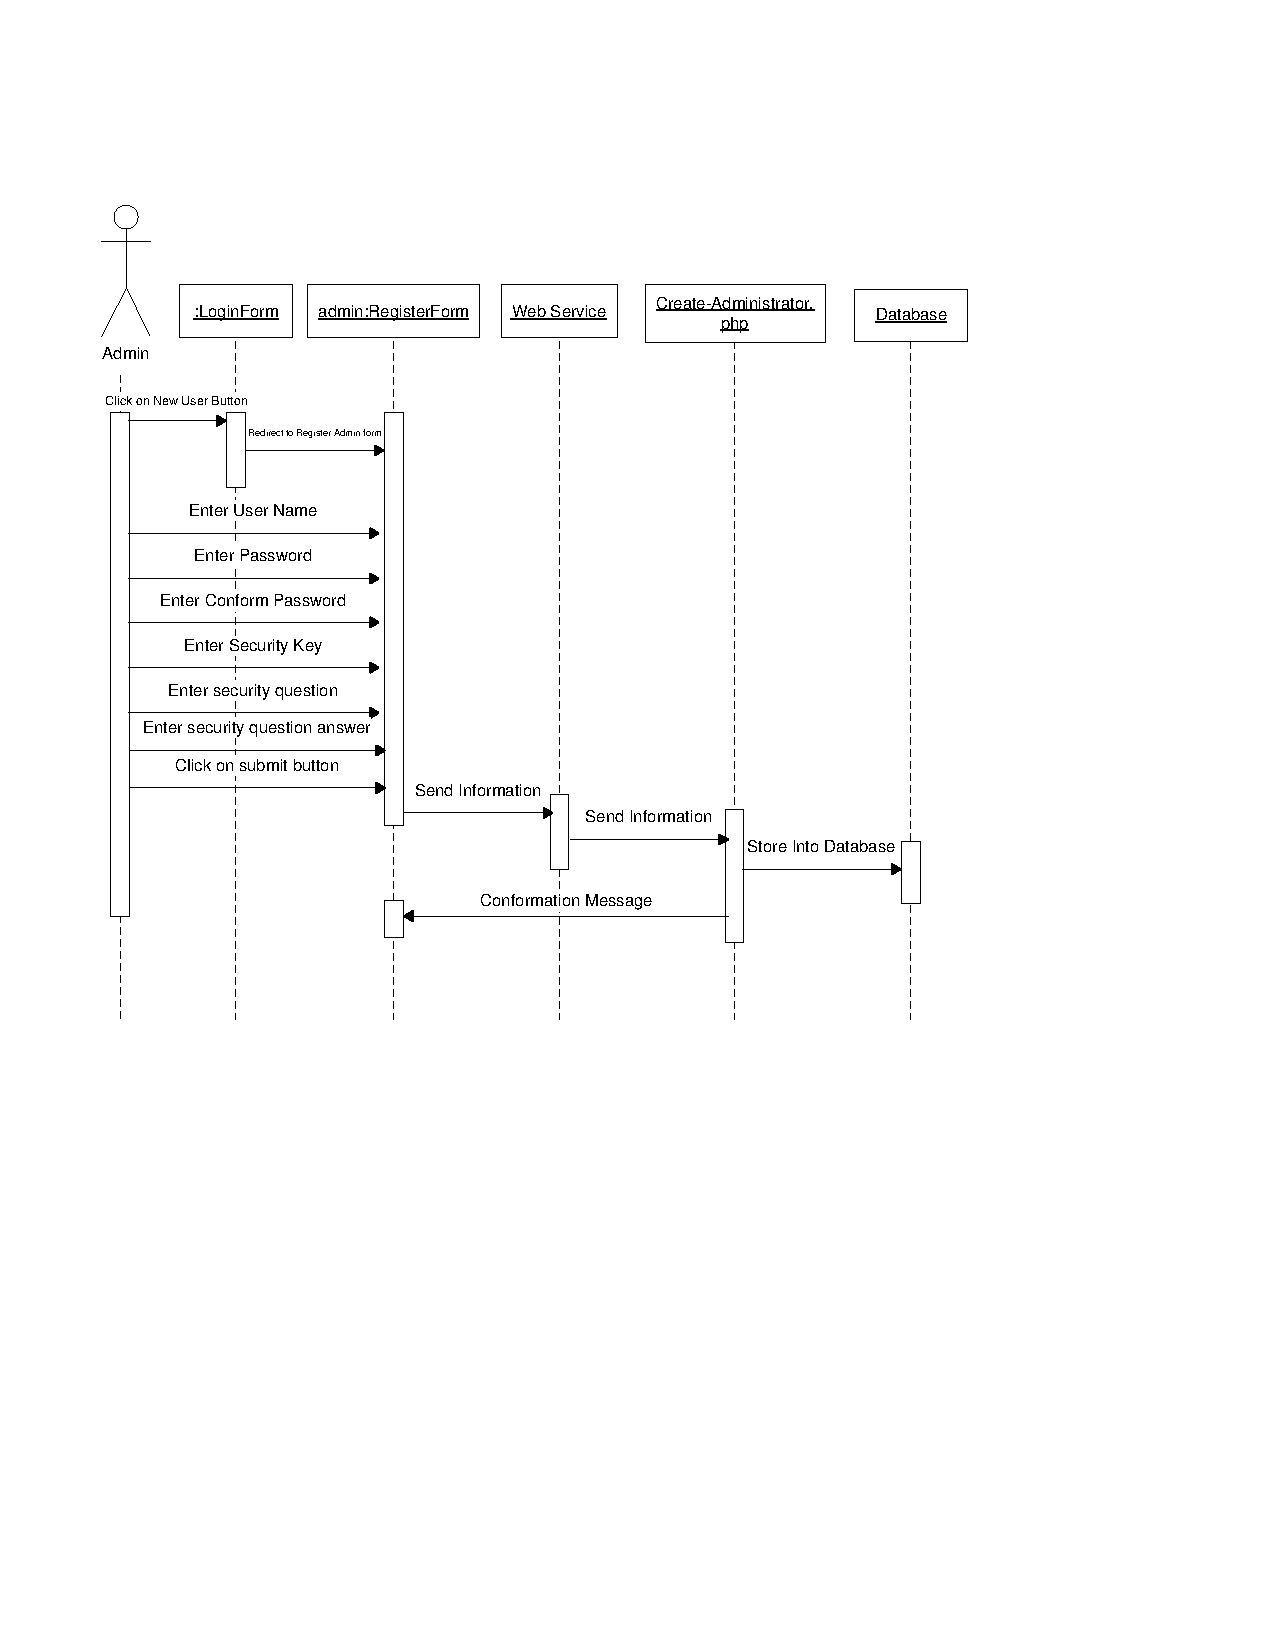
\includegraphics[width=5in]
{SDforRegisterAdmin1.pdf}
\caption{sequence diagram for Admin Registration.}
\end{figure}

Above diagram shows sequence diagram for admin registration. Admin gives required information as well as key. The username and password is used for further application. The whole data is saved into database.

\subsection{Sequence Diagrams for Register Staff:}
\begin{figure}[H]

\centering

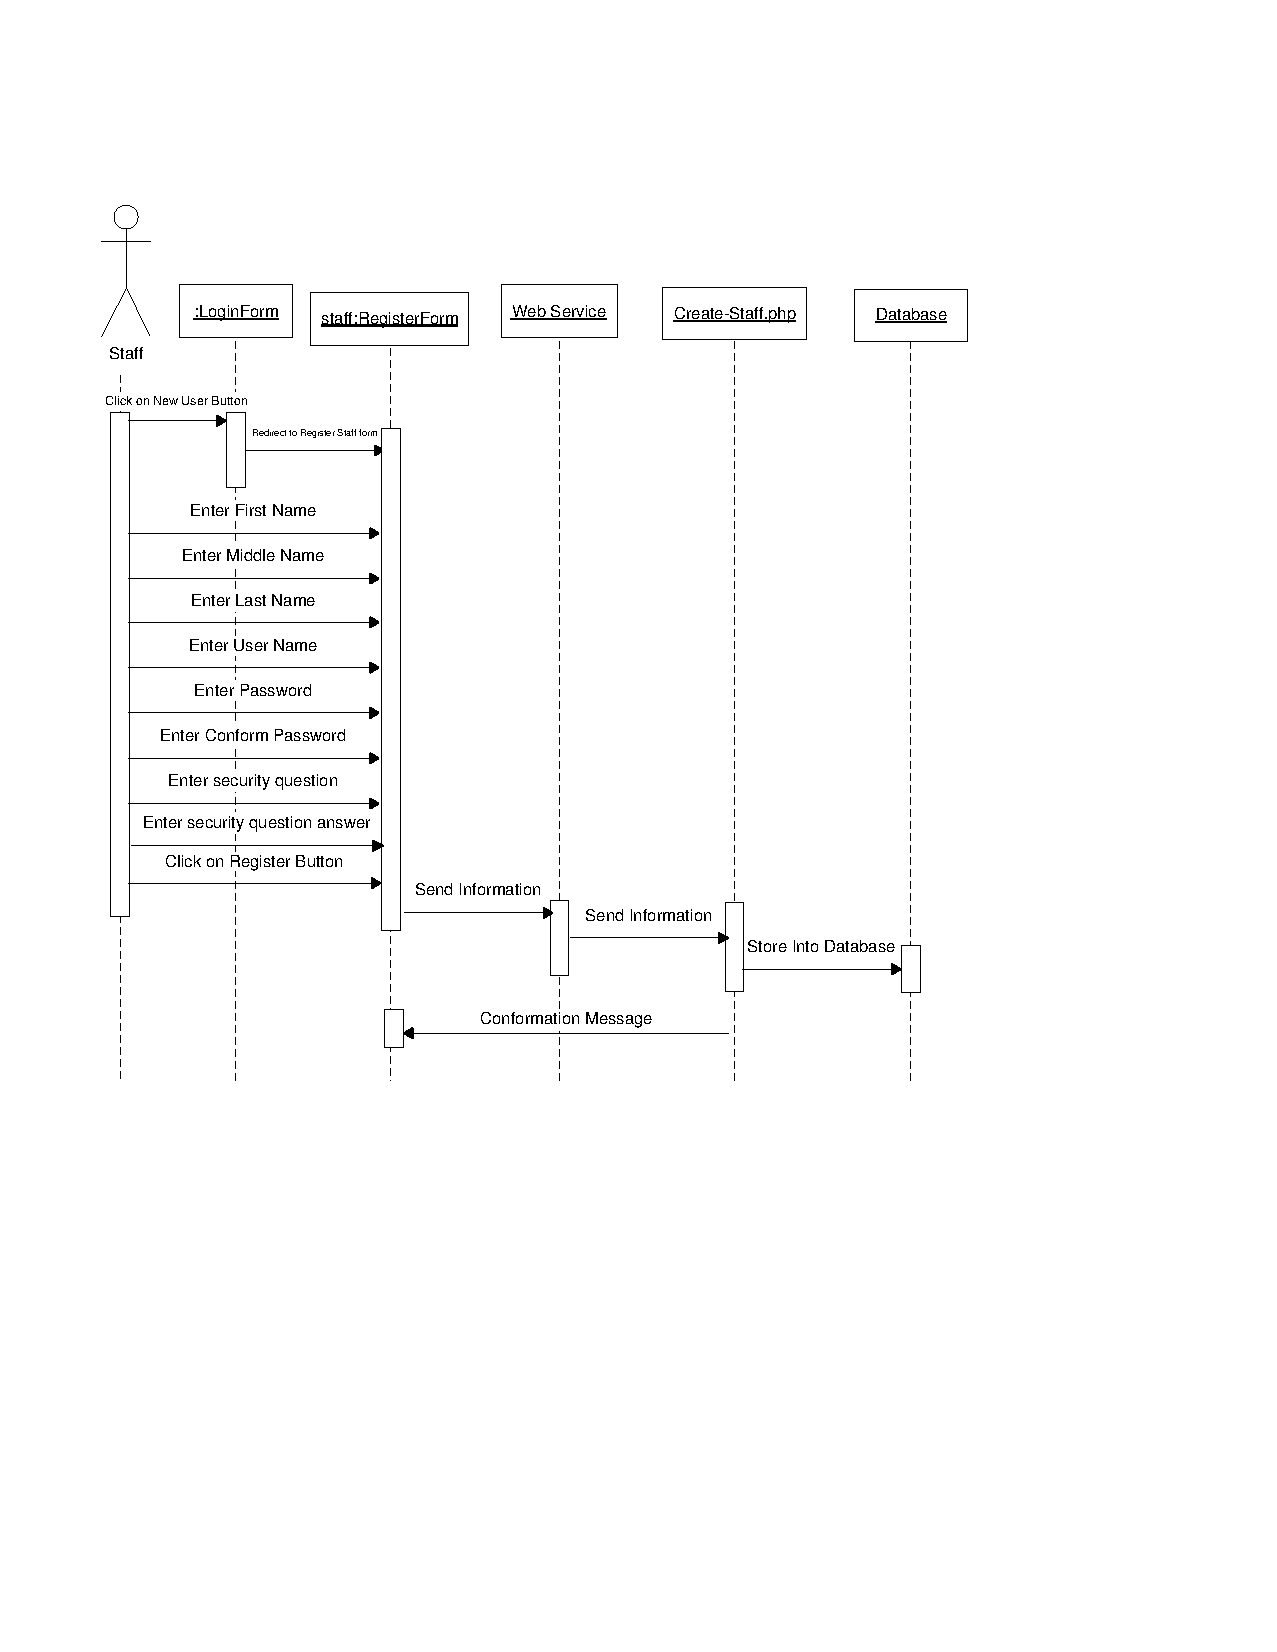
\includegraphics[width=5in]
{SDforRegisterStaff1.pdf}
\caption{sequence diagram for Staff Registration.}
\end{figure}

Above diagram shows sequence diagram for staff registration. Staff gives required information in form. The username and password is used for further application. The whole data is saved into database.

\subsection{Sequence Diagrams for Register Student:}
\begin{figure}[H]

\centering

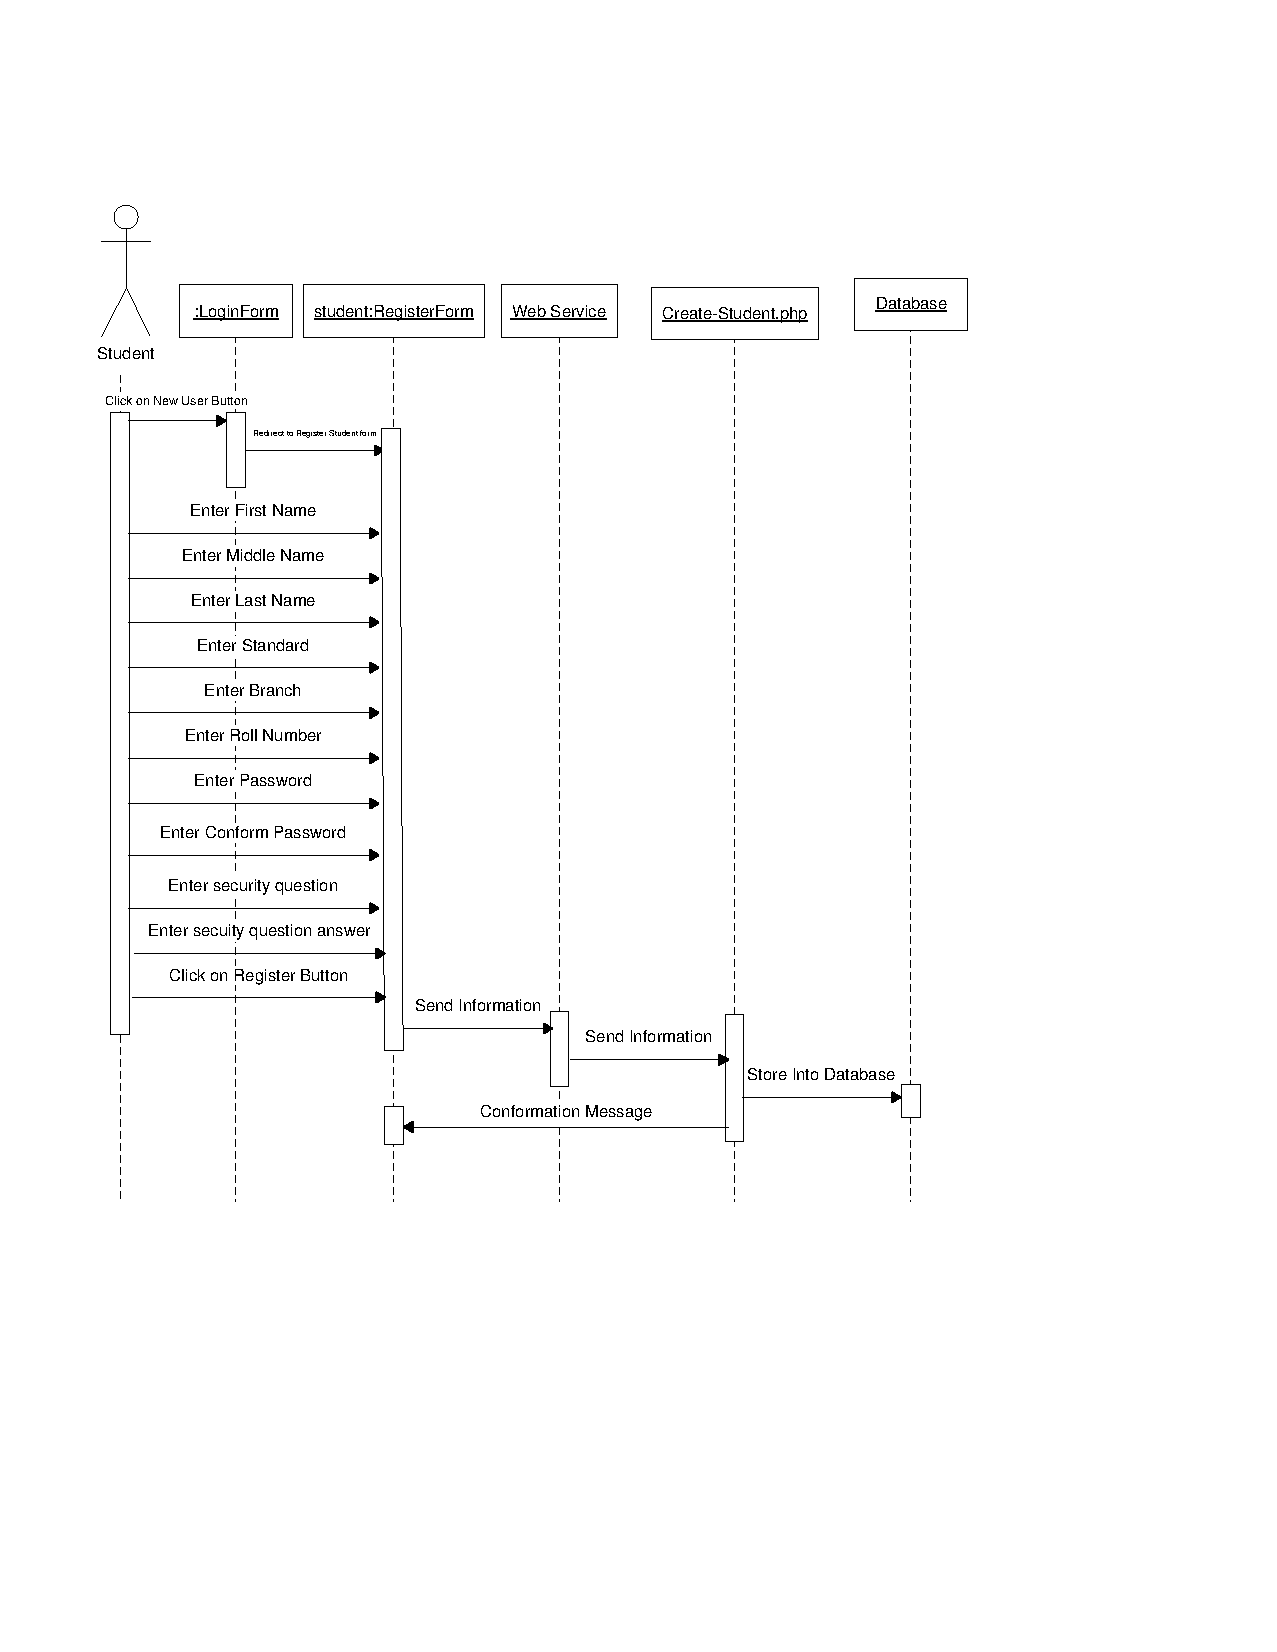
\includegraphics[width=5in]
{SDforRegisterStudent1.pdf}
\caption{sequence diagram for Student Registration.}
\end{figure}

Above diagram shows sequence diagram for student registration. Student gives required information in form. The username and password is used for further application. The whole data is saved into database.

\subsection{Sequence Diagrams for View Video:}
\begin{figure}[H]

\centering

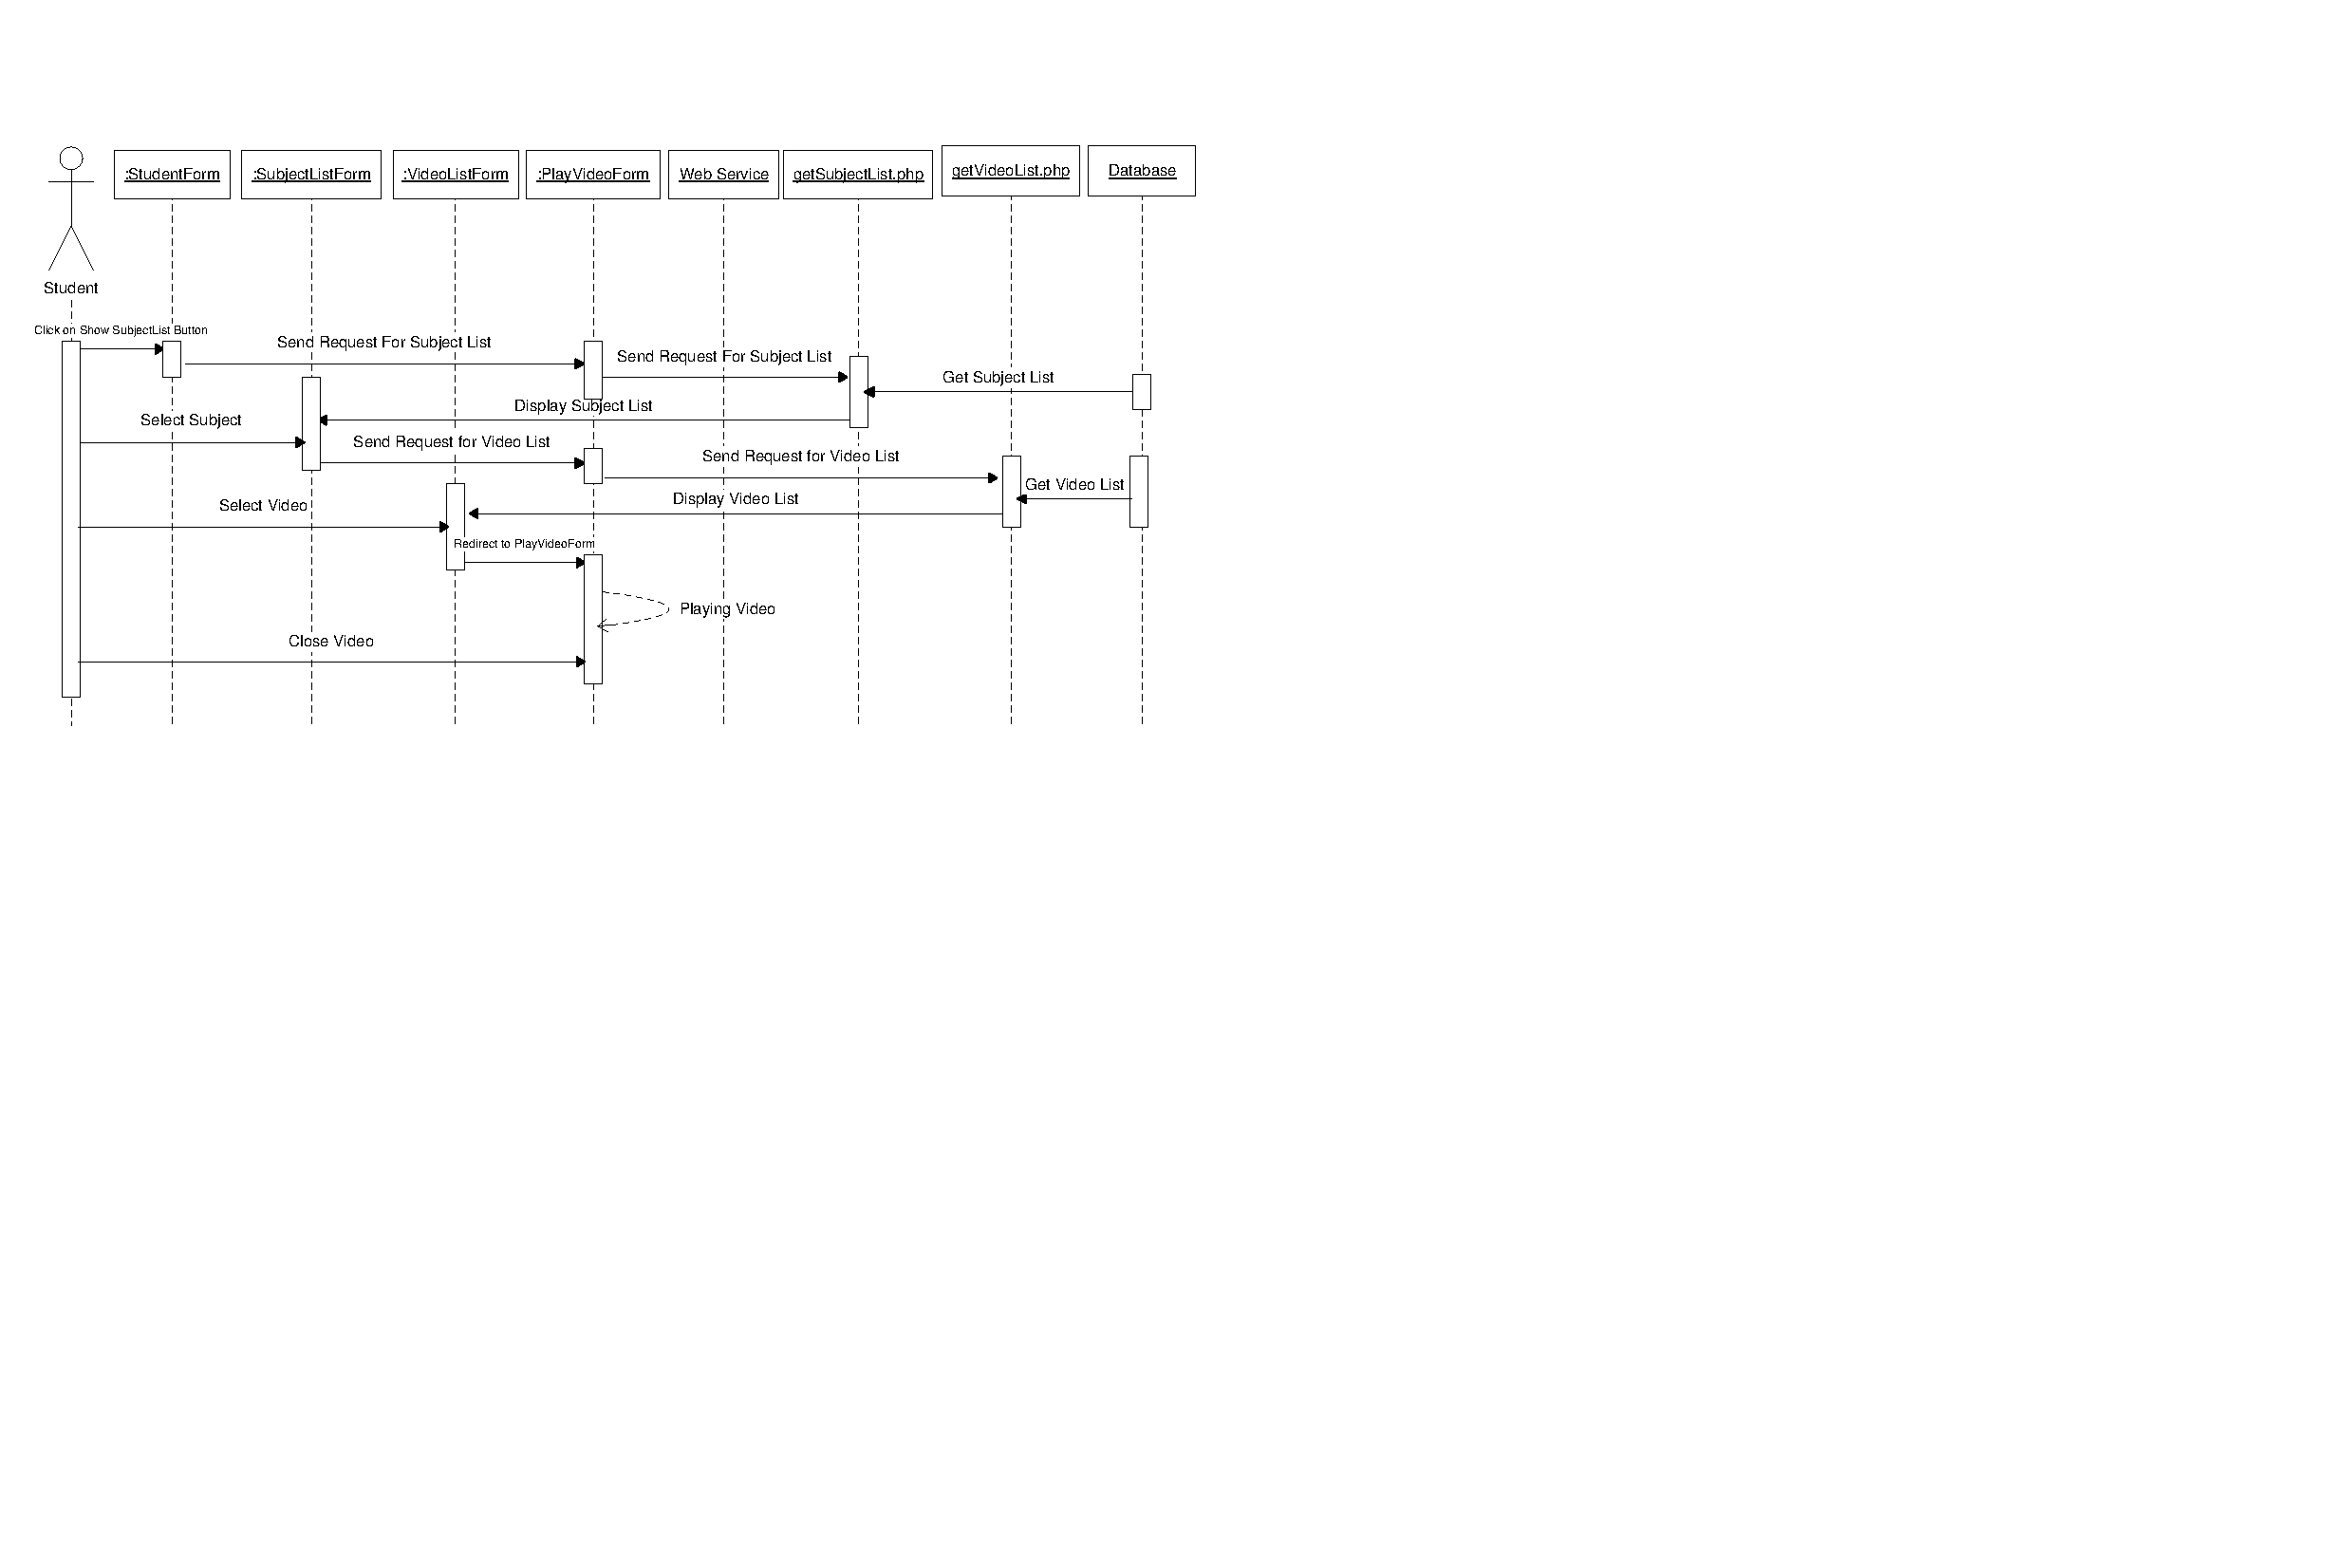
\includegraphics[width=5in]
{SDForViewVideo1.pdf}
\caption{sequence diagram for View Video.}
\end{figure}

The above figure indicates the sequence diagram for view video. When authorized student wants videos then first he/she get list of videos. By choosing the particular video, he/she can able to do the pause video, resume video or closing video.

\subsection{Sequence Diagrams for Bookmark Video:}
\begin{figure}[H]

\centering

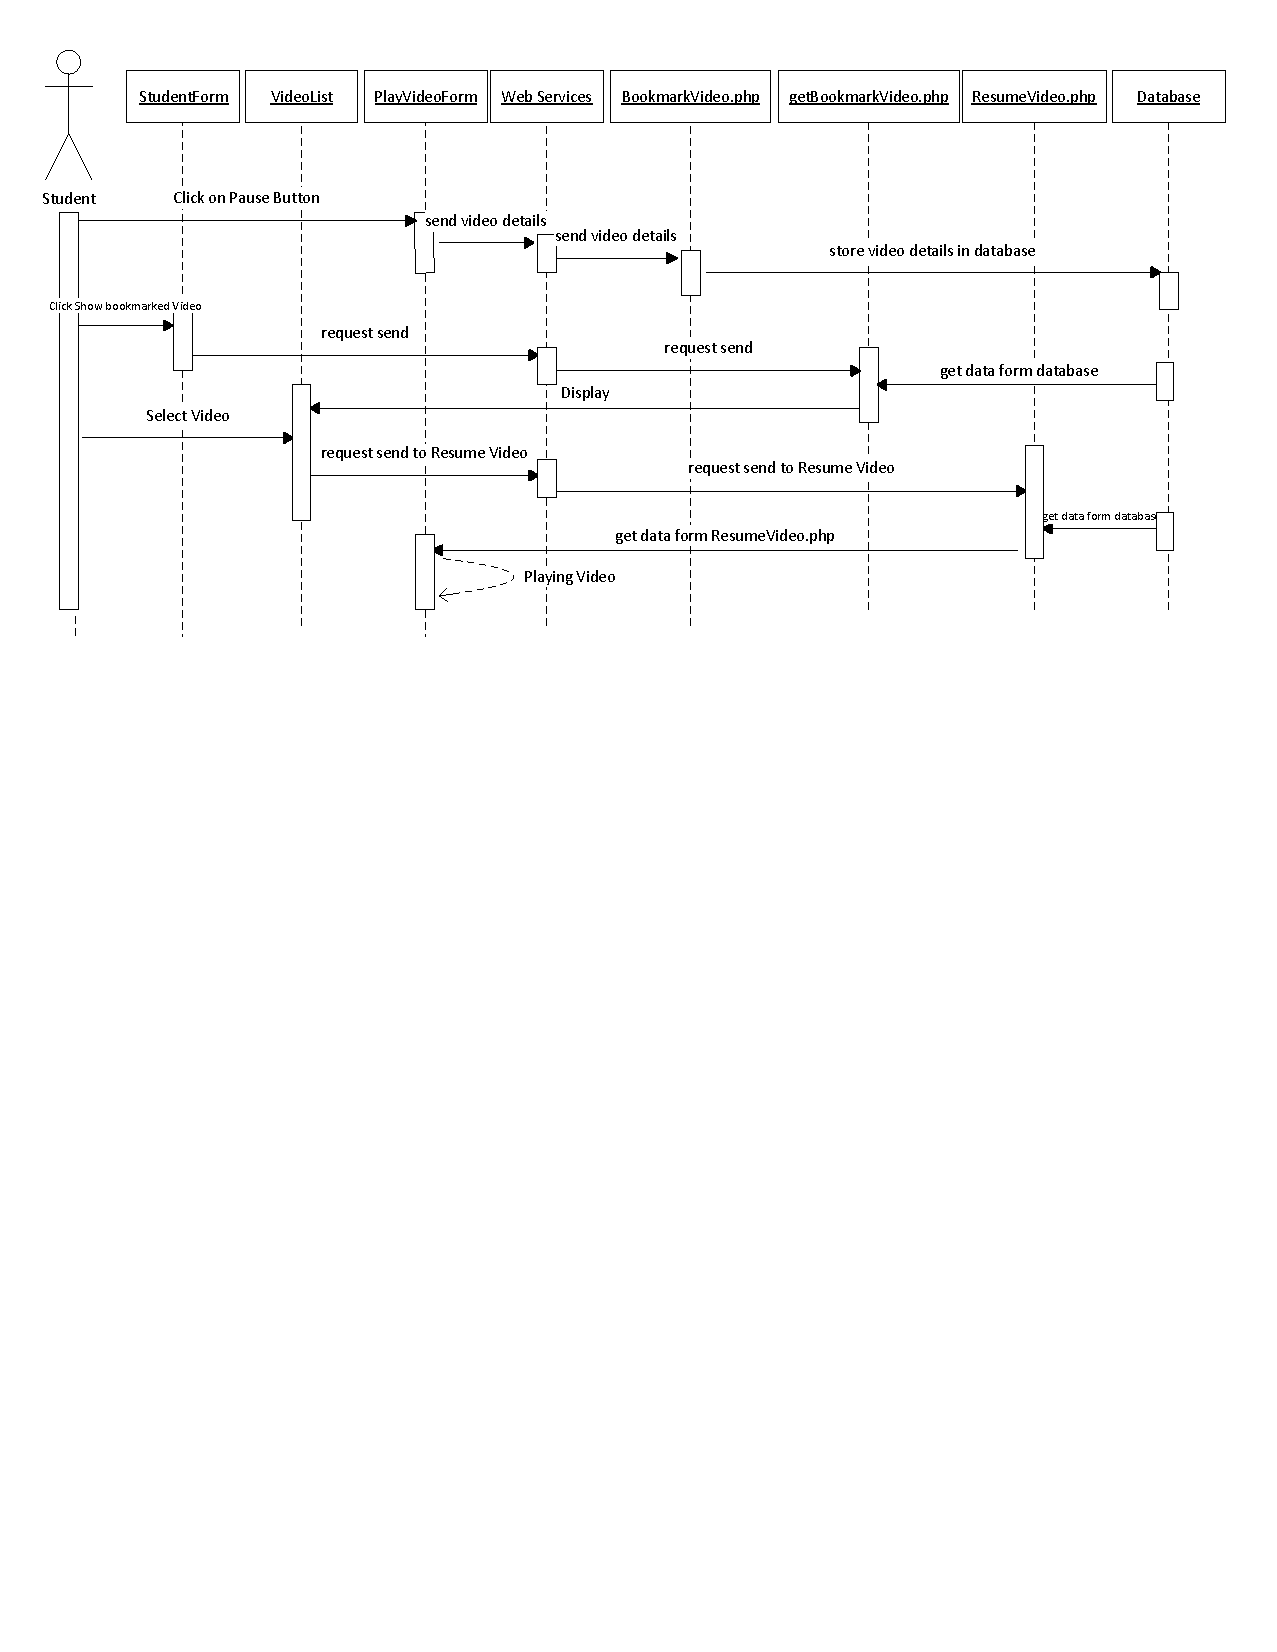
\includegraphics[width=5in]
{bookmark1.pdf}
\caption{sequence diagram for Bookmark Video.}
\end{figure}

The above figure indicates the sequence diagram for Bookmark video. When authorized student pause the video then remaining time and  pause time is stored into the bookmark history database. When next time student login, he\slash she can able to resume previously paused video.


\subsection{Sequence Diagrams for Upload Video:}
\begin{figure}[H]

\centering

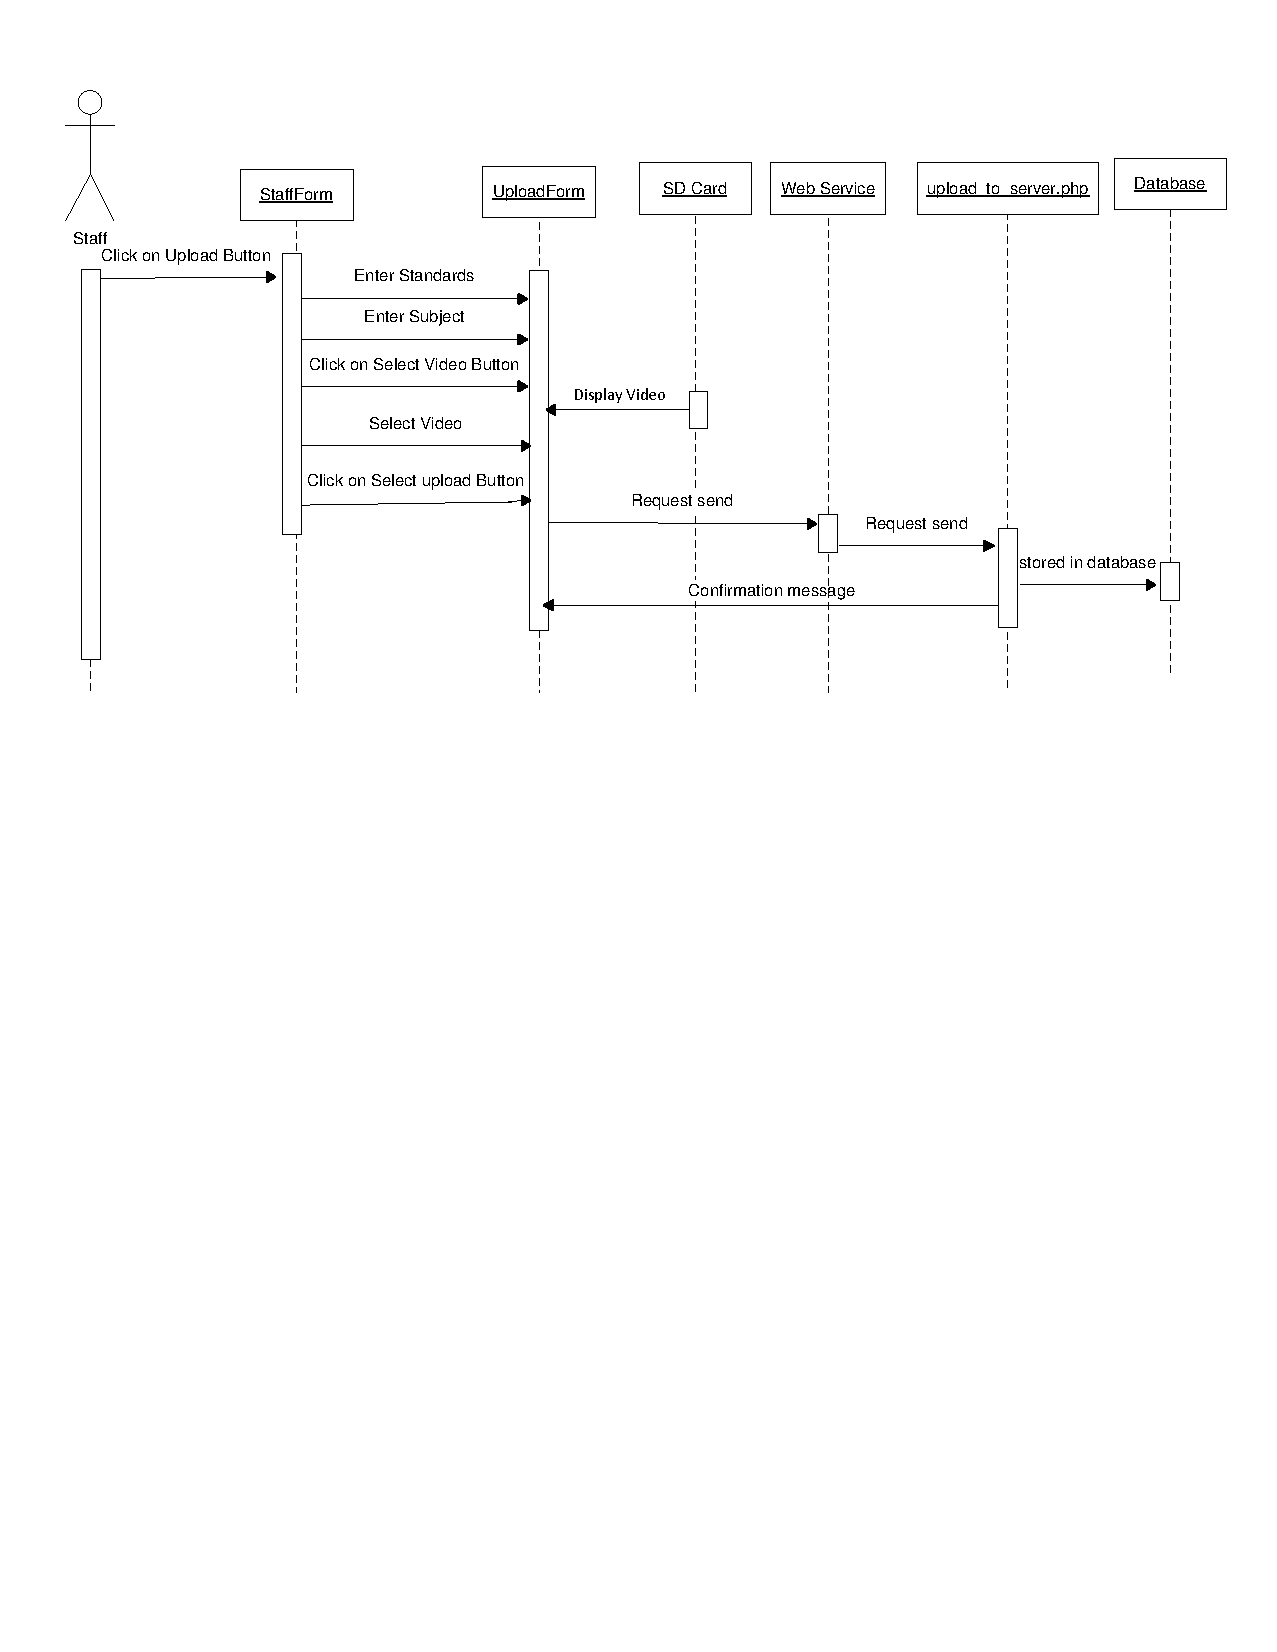
\includegraphics[width=5in]
{uploadVideo1.pdf}
\caption{sequence diagram for Upload Video.}
\end{figure}

The above figure indicates the sequence diagram for Upload video. When staff get login the system he can upload the video. The uploaded video is saved into database.

\subsection{Sequence Diagrams for Record Video:}
\begin{figure}[H]

\centering

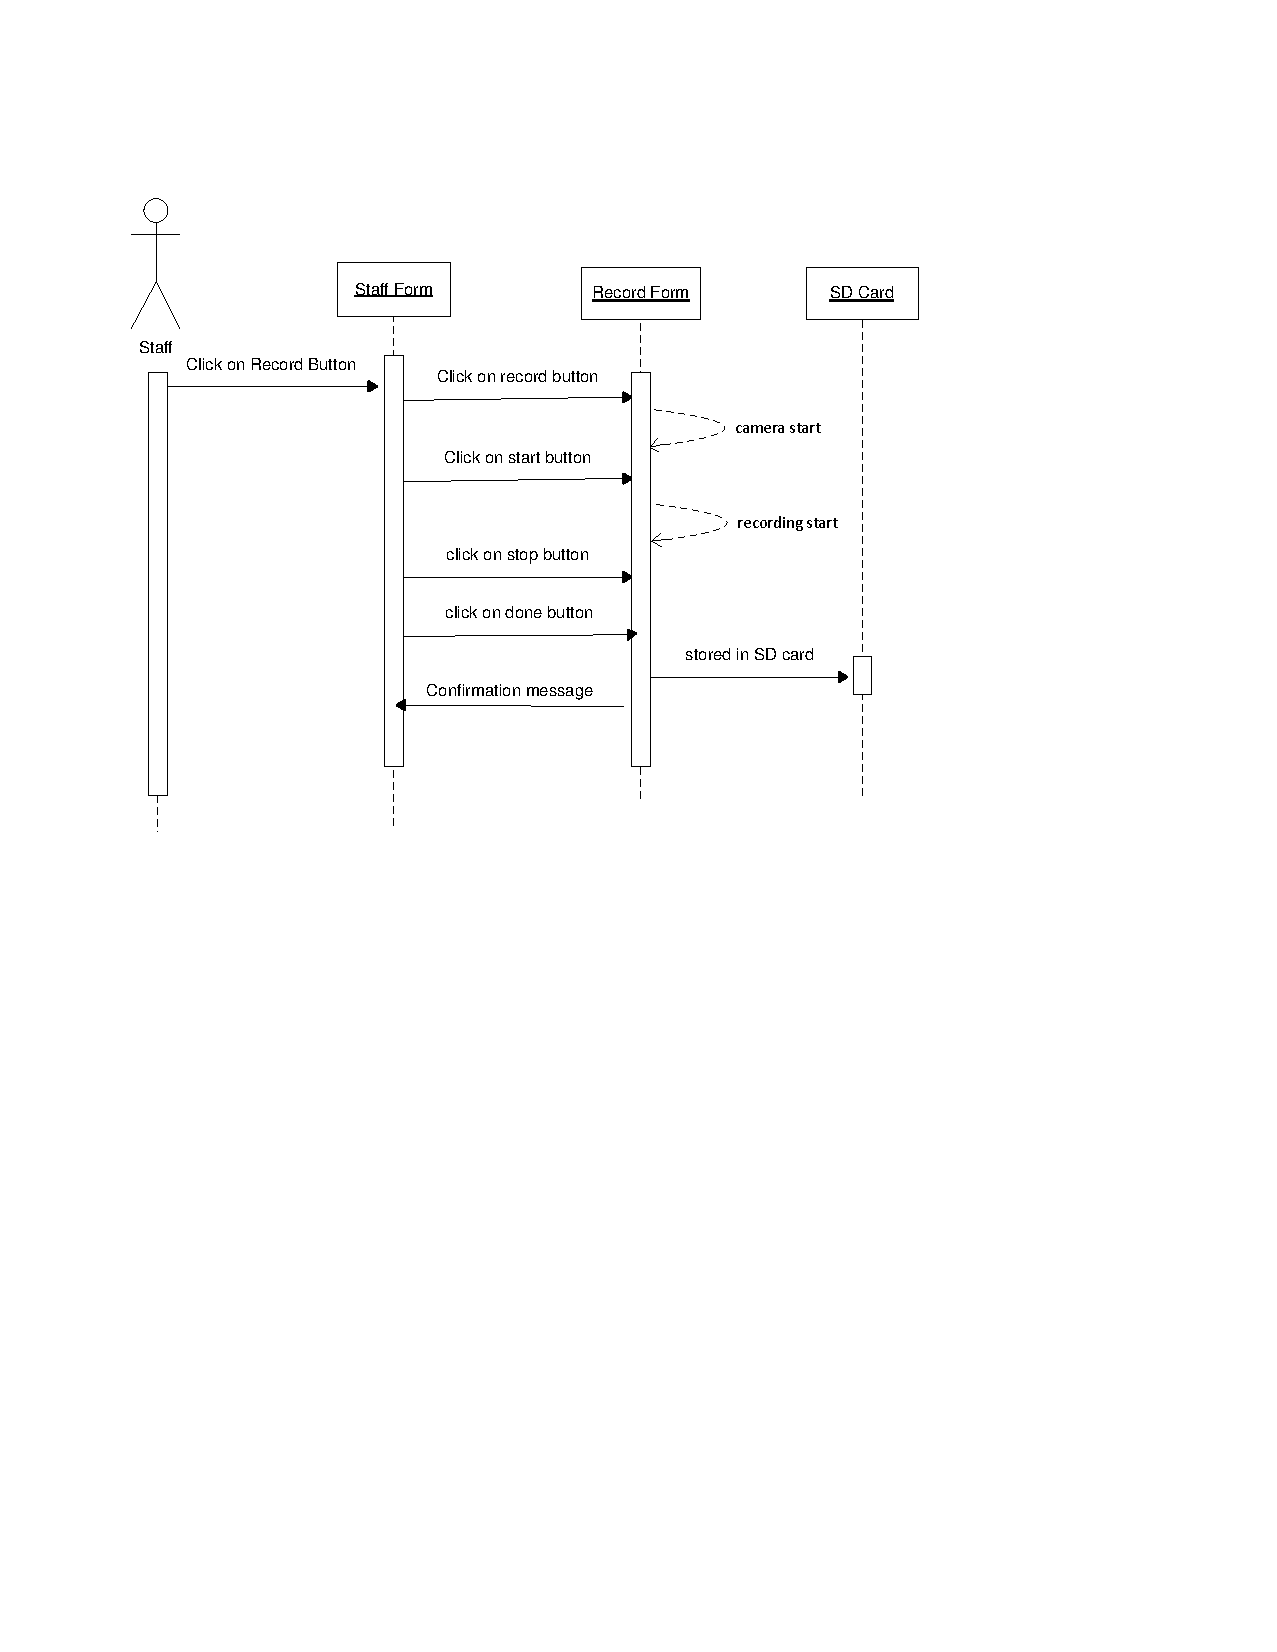
\includegraphics[width=5in]
{recordVideo1.pdf}
\caption{sequence diagram for Record Video.}
\end{figure}

The above figure indicates the sequence diagram for record video.When staff get login the system he can record the video.The staff can also upload the recorded video.The recorded video is saved into database.


\subsection{Sequence Diagrams for Delete Video:}
\begin{figure}[H]

\centering

\includegraphics[width=5in]
{deleteVideo1.pdf}
\caption{sequence diagram for Delete Video.}
\end{figure}

The above figure indicates the sequence diagram for delete video. Admin has authority to delete video from database.


\section{Class Diagram}

A UML class diagram describes the object and information structures used by your application, both internally and in communication with its users. It describes the information without reference to any particular implementation. Its classes and relationships can be implemented in many ways, such as database tables, XML nodes, or compositions of software objects.

{\bfseries Components of class diagram:}
\begin{enumerate}
\item Class:

A definition of objects that share given structural or behavioral characteristics.

\item  Attribute:

A typed value attached to each instance of a classifier.

\item Operation:

A method or function that can be performed by instances of a classifier.
\end{enumerate}

 \subsection{Class Diagram:}
\begin{figure}[H]

\centering

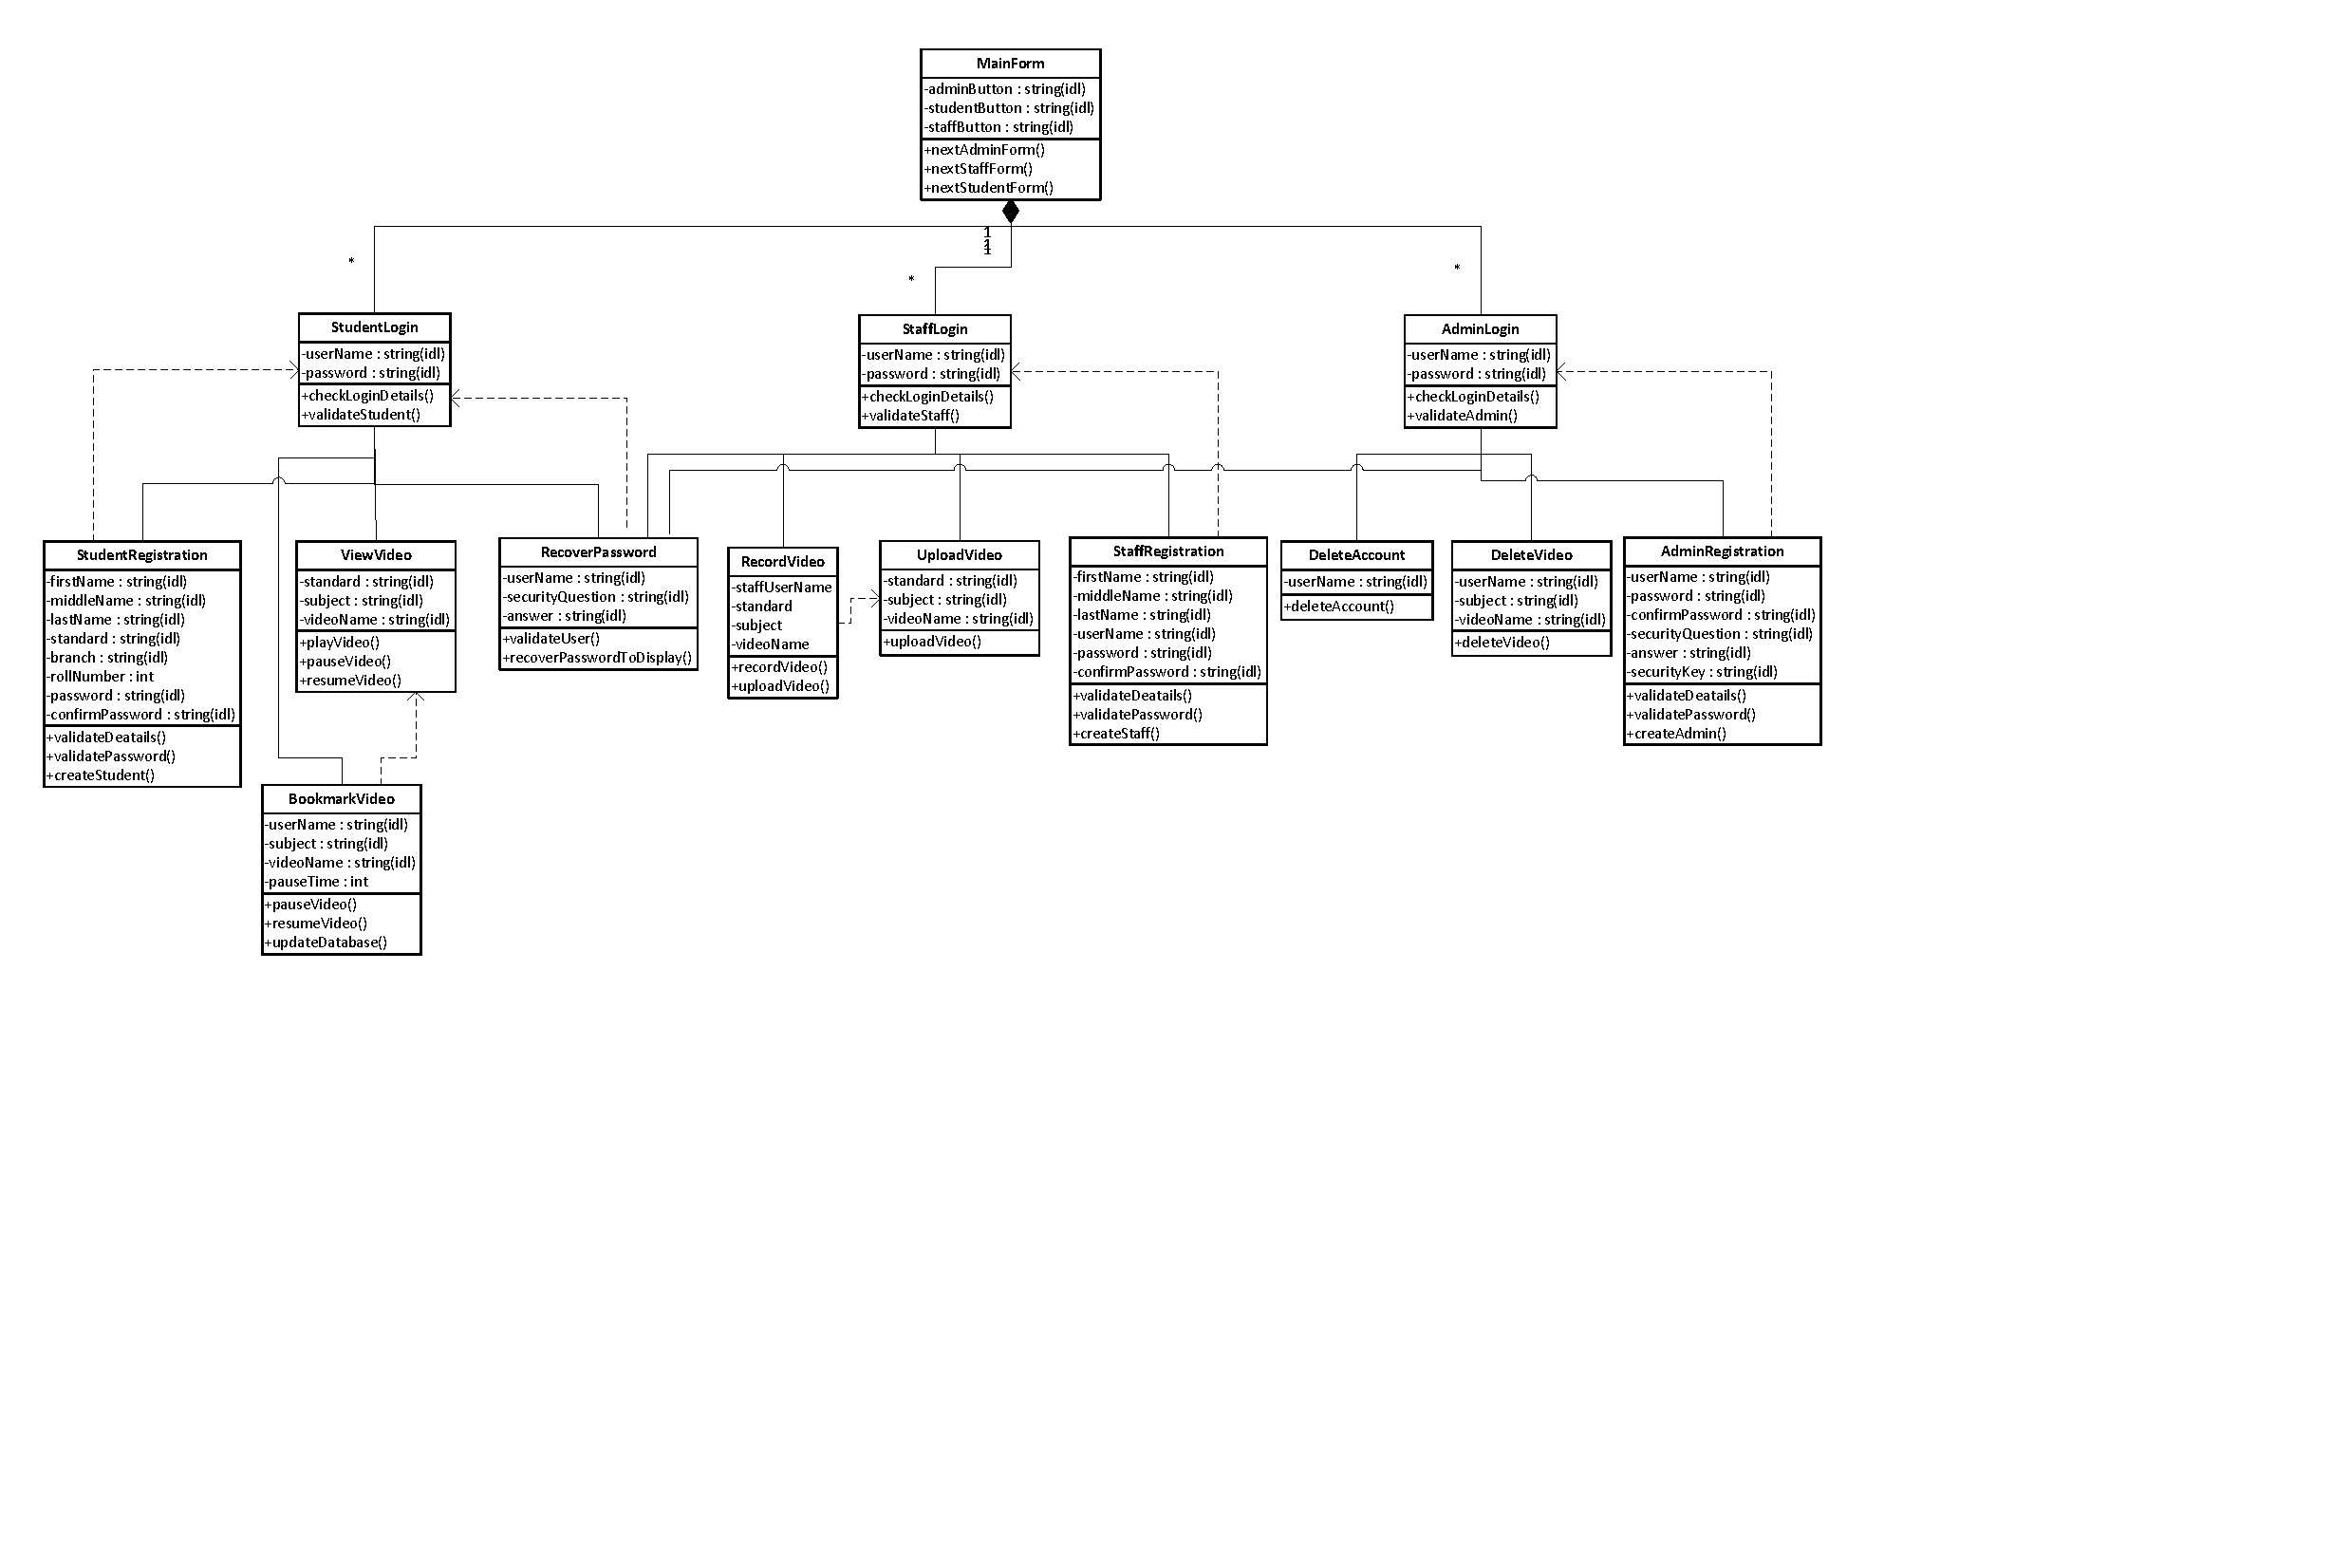
\includegraphics[width=5in]
{ClassDiagram1.pdf}
\caption{Class diagram for Virtual Classroom.}
\end{figure}

\section{Deployment Diagram:}

A deployment diagram in the Unified Modeling Language models the physical deployment of artifacts on nodes.To describe a web site, for example, a deployment diagram would show what hardware components (nodes) exist (e.g., a web server, an application server, and a database server), what software components (artifacts) run on each node (e.g., web application, database), and how the different pieces are connected (e.g. JDBC, REST, RMI).
The nodes appear as boxes, and the artifacts allocated to each node appear as rectangles within the boxes. Nodes may have sub nodes, which appear as nested boxes. A single node in a deployment diagram may conceptually represent multiple physical nodes, such as a cluster of database servers.

{\bfseries There are two types of Nodes:}
\begin{enumerate}
\item Device Node.
\item Execution Environment Node.
\end{enumerate}

Device nodes are physical computing resources with processing memory and services to execute software, such as typical computers or mobile phones. An execution environment node (EEN) is a software computing resource that runs within an outer node and which itself provides a service to host and execute other executable software elements

 \subsection{Deployment Diagram:}
\begin{figure}[H]

\centering

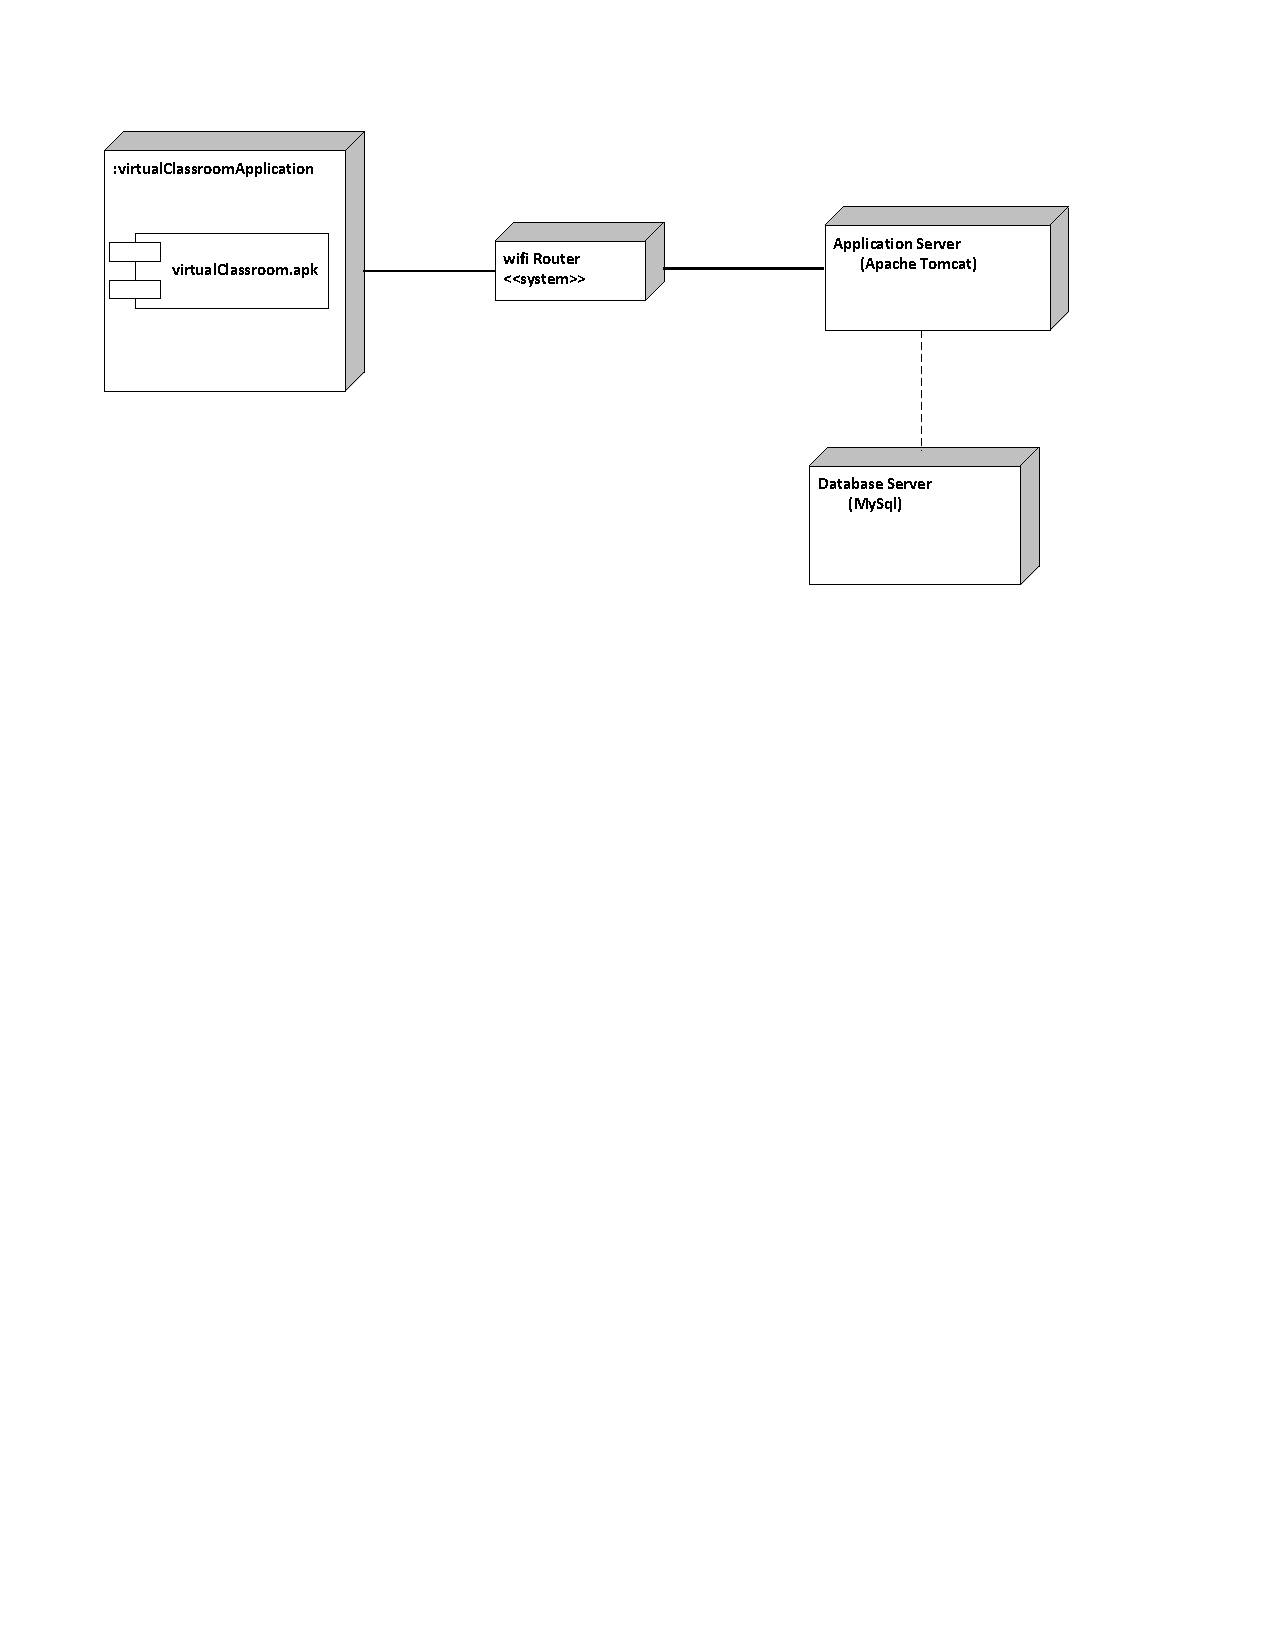
\includegraphics[width=5in]
{Deployment1.pdf}
\caption{Deployment diagram for Virtual Classroom.}
\end{figure}
